\textbf{\textit{Results}}---
\begin{figure}[t!]
    \centering
    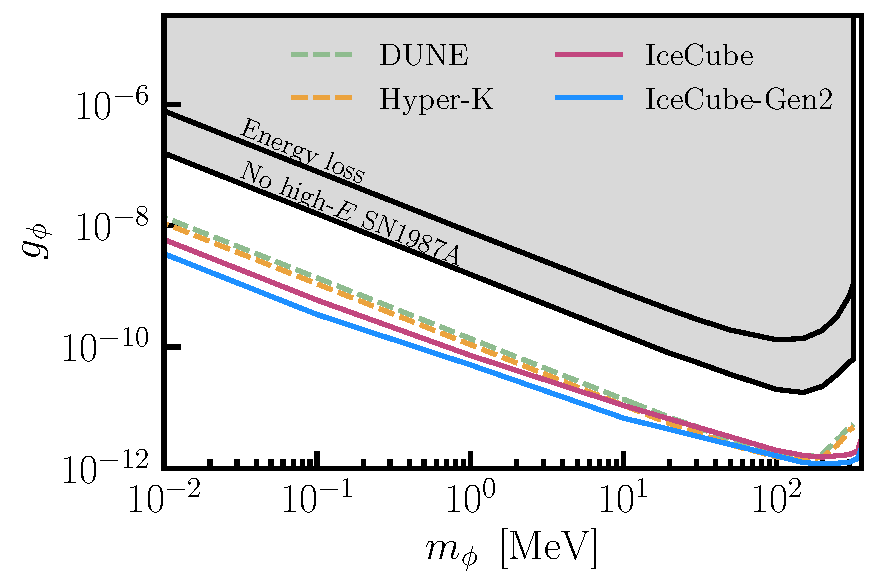
\includegraphics[width=0.47\textwidth]{figures/majoran_sensitivity}
    \caption{\textbf{\textit{Exclusion sensitivities for the Majoron case.}}
    The lines on this plot show the exclusion sensitivity for IceCube, and two next-generation neutrino experiments, Hyper-Kamiokande and DUNE.
    Additionally, we also show the reaches by SN cooling (blue) and by the lack of observation of high-energy neutrinos from SN1987A (grey) \cite{Fiorillo:2022cdq}, with the width of the lines quantifying uncertainties from SN modeling.
    }
    \label{fig:sensitivity}
\end{figure}
Looking for rapid raises within various time windows at neutrino telescope in the occurrence of future nearby SN explosion will provide exceptional tests of the parameter space. Assuming the SN event happens in the galaxy at a distance $D_{\rm SN}=\unit[10]{kpc}$, which is not unlikely~\cite{Reed:2005en,Rozwadowska:2020nab}, we consider the currently operating IceCube neutrino observatory as an example. 
The expected exclusion limit are shown in \cref{fig:sensitivity} (dark red) if no excess of hits on top of those from background noise and the standard neutrino flux were observed. JUNO expected to start taking data soon, while DUNE and Hyper-K requiring longer time to start operating, will be able to test the parameter of Majorons by looking for high energy neutrino following \cite{Fiorillo:2022cdq} if such SN event happens during their operation time. We present the estimated reaches of JUNO, DUNE and Hyper-K in \cref{fig:sensitivity} as xxx, red and orange lines, respectively, leaving aside careful detector analysis, together with current limits \cite{Fiorillo:2022cdq} from the aforementioned energy loss requirement (blue band), and non-observation of high energy neutrinos from SN 1987A (gray band) in \cref{fig:sensitivity}. 

We observe that while for the intermediate mass region, the constraints from IceCube are comparable to that from DUNE and Hyper-K, at both low mass region $m_\phi \lesssim \unit[10]{MeV}$ and high mass region $m_\phi \gtrsim \unit[200]{MeV}$, IceCube can provide stronger constraints. This is the outcome we expect. For light $\phi$ case with negligible time delay, the neutrino signals can  arrive at the detector even before the peak of standard neutrino flux arrives. The resulting hits would appear in a time window separated from that when most of standard flux contribution appears, as we show in the left panel of \cref{fig:hits_and_likelihood}, thus enhancing the reaches. On the high mass end, neutrino signals will arrive much later than the standard case, where a time window at late time can be considered to reduce the standard neutrino contaminations. 

Uncertainties on the analysis from different modeling SN explosion are minor, as studies in \cite{li2023old} and potential discrepancies between data and modeling are unresolved questions. Nevertheless we point out that the discrepancy could be within $2\sigma$ level which will only change our exclusion limit by a small factor.

\textbf{\textit{Outlook}}---
we can also study axion cases, mixing cases with this strategy. Pre-supernova bouncing.

\begin{acknowledgments}
We would like to thank xxx for stimulating discussions about this work. Y.-Y. L is supported by the NSF of China through Grant
No. 12247103 and Grant No. xxx.
\end{acknowledgments}
